\documentclass[a4paper]{article}
\usepackage[utf8]{inputenc}
\usepackage[spanish, es-tabla, es-noshorthands]{babel}
\usepackage[table,xcdraw]{xcolor}
\usepackage[a4paper, footnotesep = 1cm, width=20cm, top=2.5cm, height=25cm, textwidth=18cm, textheight=25cm]{geometry}
%\geometry{showframe}

\usepackage{tikz}
\usepackage{amsmath}
\usepackage{amsfonts}
\usepackage{amssymb}
\usepackage{float}
\usepackage{graphicx}
\usepackage{caption}
\usepackage{subcaption}
\usepackage{multicol}
\usepackage{multirow}
\setlength{\doublerulesep}{\arrayrulewidth}
\usepackage{booktabs}

\usepackage{hyperref}
\hypersetup{
    colorlinks=true,
    linkcolor=blue,
    filecolor=magenta,      
    urlcolor=blue,
    citecolor=blue,    
}

\newcommand{\quotes}[1]{``#1''}
\usepackage{array}
\newcolumntype{C}[1]{>{\centering\let\newline\\\arraybackslash\hspace{0pt}}m{#1}}
\usepackage[american]{circuitikz}
\usetikzlibrary{calc}
\usepackage{fancyhdr}
\usepackage{units} 

\graphicspath{{../Ejercicio-1/}{../Ejercicio-2/}}

\pagestyle{fancy}
\fancyhf{}
\lhead{22.67 - Señales Aleatorias}
\rhead{Lambertucci, Londero B., Moriconi, Musich, Tolaba}
\rfoot{Página \thepage}
\begin{document}
\subsection{Introducción}

El siguiente ejercicio parte de un análisis sobre el proceso aleatorio presente en la página 138 del libro selecto por la cátedra. Se realizarán simulaciones de dicho proceso y se calcularán experimentalmente la media, la varianza, la autocorrelación y el coeficiente de autocorrelación para ciertos valores de t dados y se realizará una comparación con los valores teóricos.
Luego, se.... PUNTO C 

\subsection{Valores teóricos}

El experimento que determina el proceso es la tirada de un dado no cargado y el ensamble del mismo se detalla a continuación:
\begin{equation} 
	\begin{split}
		 &y_{1} = 6 \\
		 &y_{2} = 3sin(t) \\
		 &y_{3} = -3sin(t) \\
		 &y_{4} = 3cos(t) \\
		 &y_{5} = -3cos(t) \\
		 &y_{6} = -6
	\end{split}
\end{equation}

El proceso es $Y_{(t)} = y_{i(t)}$ donde i indica el número obtenido en la tirada del dado.\\

El valor esperado teórico del proceso se obtiene de la siguiente forma:

\begin{equation*}
\begin{gathered}
	E\left[Y_{(t)}\right] = \sum_{i=1}^{6}\left( P(Y_{(t)} = y_{i(t)}) \times y_{i(t)}\right) 
\end{gathered}
\end{equation*}

Reemplazando las funciones muestra dadas y que la probabilidad $P(Y_{(t)} = y_{i(t)})= \frac{1}{6}$ $ \forall i $ obtenemos que:

\begin{equation*}
\begin{gathered}
	E\left[Y_{(t)}\right] = 0$ $\forall t 
\end{gathered}
\end{equation*}

La varianza se obtiene como:

\begin{equation*}
\begin{gathered}
	Var^{2}_{(t)} = E\left[Y_{(t)}^{2}\right]- \left(E\left[Y_{(t)}\right]\right)^{2}  = \sum_{i=1}^{6}\left( P(Y_{(t)} = y_{i(t)}) \times y_{i(t)}^{2}\right) - 0^2 = 15 $   $ \forall t 
\end{gathered}
\end{equation*}

Donde ya se obtuvo que $E\left[Y_{(t)}\right] = 0$ y 

\begin{equation*}
\begin{gathered}
	E\left[Y_{(t)}^{2}\right] = \sum_{i=1}^{6}\left( P(Y_{(t)} = y_{i(t)}) \times y_{i(t)}^{2}\right) 
\end{gathered}
\end{equation*}

Este proceso tiene media y "varianza" constantes para todo instante t.

La autocorrelación para dos instantes t1 y t2 se encuetra calculada en el libro y nos queda como:
\begin{equation*}
\begin{gathered}
	R_{xx(t_1,t_2)} = \frac{1}{6}\left(72+ 18 \cos(t_2 - t_1)\right)
\end{gathered}
\end{equation*}
Observación: El proceso tiene media constante y autocorrelación dependiente de $(t_2 - t_1)$, entonces es WSS. Por lo tanto:
\begin{equation*}
\begin{gathered}
	R_{xx(t,t)} = R_{xx(0,0)} = \frac{1}{6}\left(72+ 18 \cos(0)\right) = 15
\end{gathered}
\end{equation*}

El coeficiente de autocorrelación se obtiene con la definición del mismo:
\begin{equation*}
\begin{gathered}
	r_{xx(t_1,t_2)} = \frac{R_{xx(t_1,t_2)}-\mu_{X_{(t_1)}}^{*} \mu_{X_{(t_2)}}}{\left(R_{xx(t_1,t_1)}.R_{xx(t_2,t_2)}\right)^{1/2}} 
\end{gathered}
\end{equation*}

Como el proceso es WSS y su media es cero cualquiera sea t:

\begin{equation*}
\begin{gathered}
	r_{xx(t_1,t_2)} = \frac{R_{xx(t_1,t_2)}-0}{(R_{xx(0,0)}^2)^{1/2}} = \frac{\frac{1}{6}\left(72+ 18 \cos(t_2 - t_1)\right)}{15}
\end{gathered}
\end{equation*}

Para los instantes de t requeridos, obtenemos los siguientes resultados:
\begin{enumerate}
	\item[•]E$\left[ Y_{(\frac{\pi}{2})}\right]$= 0 
	\item[•]Var$\left[Y_{(\frac{\pi}{2})}\right]$= 15
	\item[•]$R_{xx(\frac{\pi}{4},\frac{\pi}{2})}$= $\frac{1}{6} (72 + 18 \cos(\frac{\pi}{4}))$ = 14.12132
	\item[•]$r_{xx(2\pi,\pi)} = \frac{R_{xx(\pi,2\pi)}}{15} = \frac{ (12 + 3 \cos(\pi))}{15}$ = 0.6
\end{enumerate}

\begin{equation*}
\begin{split}
	R_{YY} = & E \left\lbrace Y(t) Y(t + \tau) \right\rbrace = \frac{1}{6} \left[ 36 + 9 sin(t)sin(t + \tau) + 9 sin(t)sin(t + \tau) + 9 cos(t)cos(t + \tau) + 9 cos(t)cos(t + \tau) + 36 \right] \\
	= & \frac{1}{3} \left[ 36 + \frac{9}{2} cos(\tau) - \frac{9}{2} cos(2t + \tau) + \frac{9}{2} cos(\tau) + \frac{9}{2} cos(2t + \tau) \right] = 12 + 3 cos(\tau) = R_{YY}(\tau)
\end{split}
\end{equation*}

\begin{equation*}
\begin{split}
	\lim_{T\to\infty} < R_{YY}(\tau) >T = & \lim{T\to\infty} \frac{1}{T} \int_{-T/2}^{T/2} Y(t) Y(t + \tau) dt = \underbrace{\frac{1}{6}}{y_1(t)} \neq R{YY}(\tau) \ 	\forall \tau
\end{split}
\end{equation*}

Dado que para una de las funciones no se cumple que tienda a la autocorrelación, no es ergódico en en dicha variable.\\


\subsection{Análisis Experimental}

Para el análisis sobre los valores pedidos es necesario generar múltiples muestras sobre el proceso, en los instantes de tiempo requeridos. En primer lugar, se obtiene un número entero al azar entre 1 y 6, simulando la tirada de un dado, el cual determina qué función miembro del ensamble resulta.
A partir de la determinacion de la función correspondiente se evalua en los valores de instantes t pedidos, obteniendose:

\begin{enumerate}
   \item[•] $Y(\pi/2)$
   \item[•] $Y(\pi/4)$
   \item[•] $Y(\pi)$
   \item[•] $Y(2\pi)$
\end{enumerate}

Estos valores obtenidos se guardan como un vector. Luego, se repite el procedimiento N = 1000 veces 
y se obtiene un arreglo de vectores conteniendo muestras del proceso.
El codigo de Matlab empleado para la simulaci[on de este proceso se detalla a continuaci[on 
\\

\begin{figure}[H]
\centering
	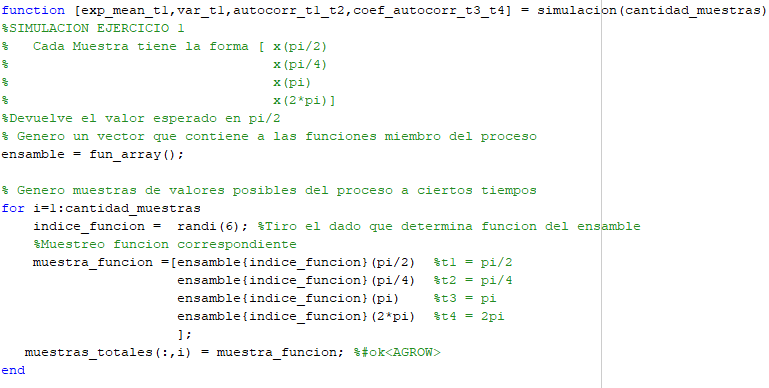
\includegraphics[width=0.8\textwidth, trim = {0 0 0 0},clip]{./ImagenesEjercicio1/main1.png}
	\caption{.}
	\label{fig:main1}
\end{figure}

Donde la funcion fun-array() designa el ensamble solicitado, el c[odigo en Matlab:

\begin{figure}[H]
\centering
	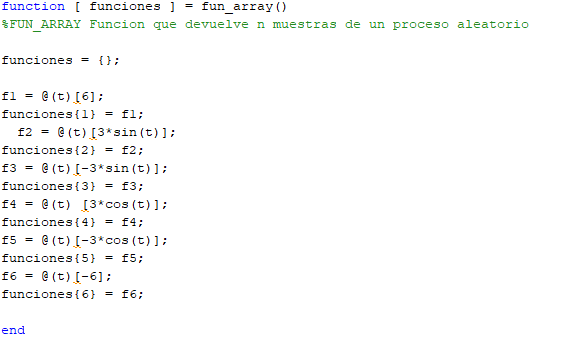
\includegraphics[width=0.6\textwidth, trim = {0 0 0 0},clip]{./ImagenesEjercicio1/fun_array.png}
	\caption{.}
	\label{fig:fun_array}
\end{figure}

A continuación, por ejemplo se muestran los resultados para $Y(\pi/2)$ para N = 100 experimentos realizados.

\begin{figure}[H]
\centering
	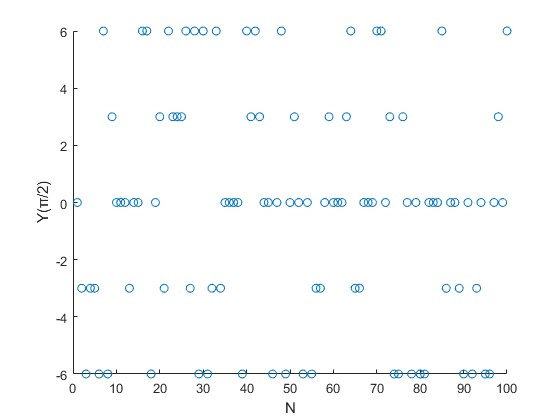
\includegraphics[width=0.4\textwidth, trim = {0 0 0 0},clip]{./ImagenesEjercicio1/ypi_2.png}
	\caption{.}
	\label{fig:ypi_2}
\end{figure}

También para $Y(\pi/4)$.

\begin{figure}[H]
\centering
	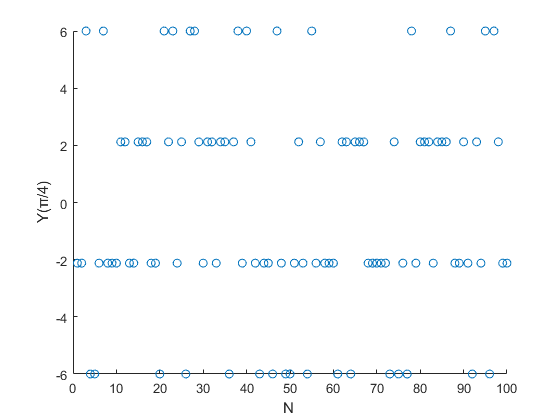
\includegraphics[width=0.4\textwidth, trim = {0 0 0 0},clip]{./ImagenesEjercicio1/ypi_4.png}
	\caption{.}
	\label{fig:ypi_4}
\end{figure}

Observaci[on: En las Figuras (\ref{fig:ypi_2}) y (\ref{fig:ypi_4}) se puede "estimar" visualmente que la media para el proceso es cero. 
\\
Luego, se calculan promediando los valores pedidos con el código:

\begin{figure}[H]
\centering
	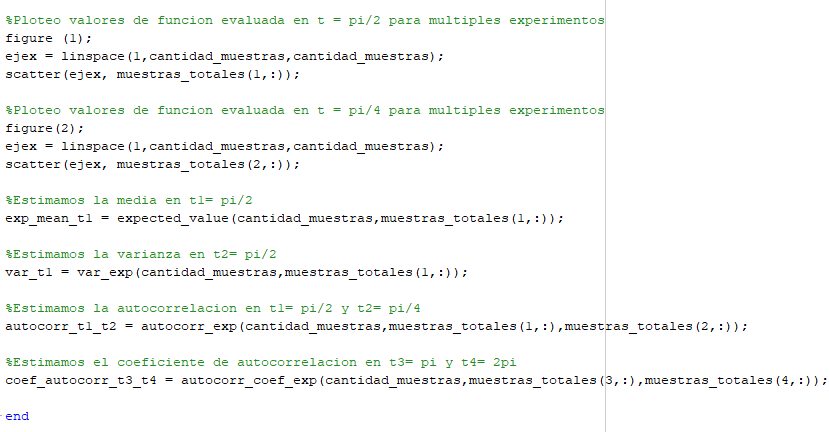
\includegraphics[width=0.8\textwidth, trim = {0 0 0 0},clip]{./ImagenesEjercicio1/main2.png}
	\caption{.}
	\label{fig:main2}
\end{figure}

Detallando cada función:
\begin{enumerate}
\item[•] La funcio[n estimadora de la media en $t = \frac{\pi}{2}$, E$\left[ Y_{(\frac{\pi}{2})}\right]$
\begin{figure}[H]
\centering
	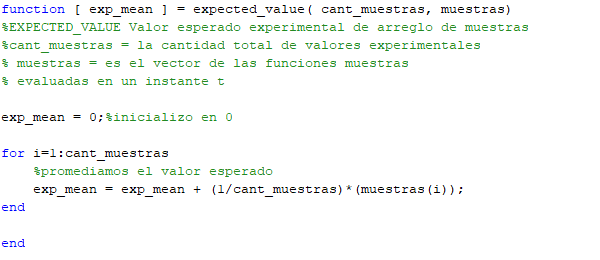
\includegraphics[width=0.6\textwidth, trim = {0 0 0 0},clip]{./ImagenesEjercicio1/expval.png}
	\caption{.}
	\label{fig:expval}
\end{figure}

\item[•] La función estimadora de la varianza en $t = \frac{\pi}{2}$, Var$\left[Y_{(\frac{\pi}{2})}\right]$
\begin{figure}[H]
\centering
	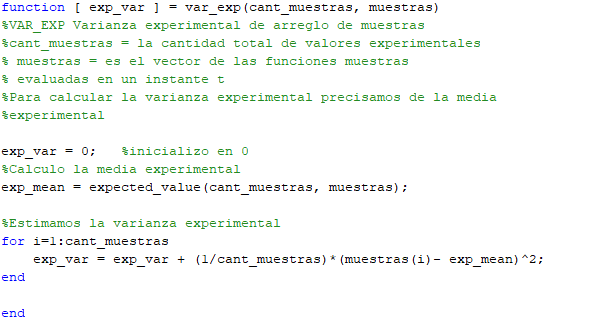
\includegraphics[width=0.6\textwidth, trim = {0 0 0 0},clip]{./ImagenesEjercicio1/expvar.png}
	\caption{.}
	\label{fig:expvar}
\end{figure}

\item[•] La función estimadora de la autocorrelación en $t_1 = \frac{\pi}{4}$ y $t_2 = \frac{\pi}{2}$, $R_{xx(\frac{\pi}{4},\frac{\pi}{2})}$
\begin{figure}[H]
\centering
	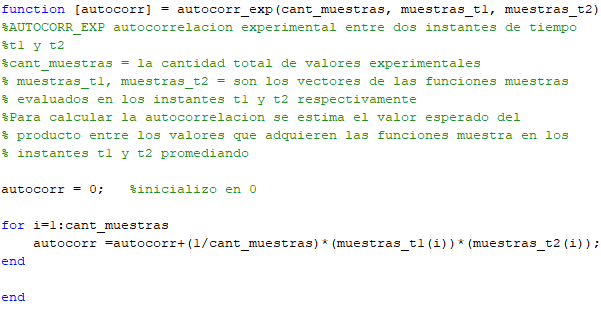
\includegraphics[width=0.6\textwidth, trim = {0 0 0 0},clip]{./ImagenesEjercicio1/autocorr.png}
	\caption{.}
	\label{fig:autocorr}
\end{figure}

\item[•] La función estimadora del coeficiente de autocorrelación en $t_3 = \frac{2\pi}{4}$ y $t_4 = \pi$, $r_{xx(2\pi,\pi)}$
\begin{figure}[H]
\centering
	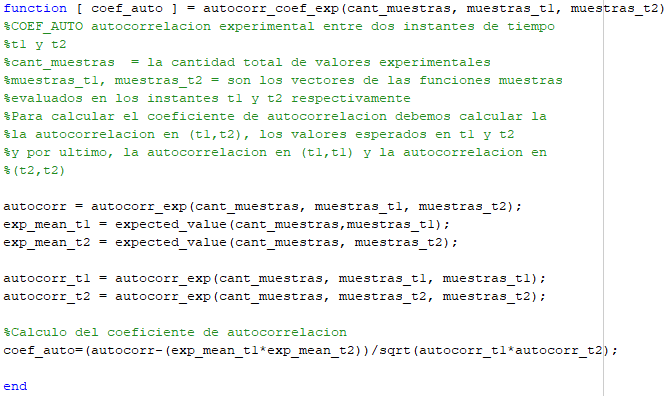
\includegraphics[width=0.6\textwidth, trim = {0 0 0 0},clip]{./ImagenesEjercicio1/coefauto.png}
	\caption{.}
	\label{fig:coefauto}
\end{figure}
\end{enumerate}

Corriendo la simulación para N = 1000, se arrojaron los siguientes resultados:
\begin{figure}[H]
\centering
	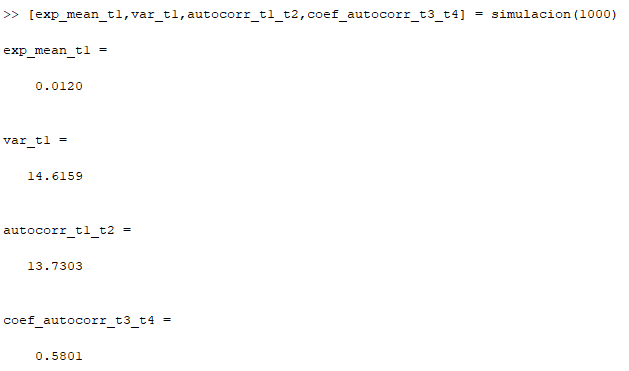
\includegraphics[width=0.6\textwidth, trim = {0 0 0 0},clip]{./ImagenesEjercicio1/result.png}
	\caption{.}
	\label{fig:result}
\end{figure}

Observando la figura (\ref{fig:result}) obtenemos que:
\begin{enumerate}
	\item[•]E$\left[ Y_{(\frac{\pi}{2})}\right]$= 0.0120 
	\item[•]Var$\left[Y_{(\frac{\pi}{2})}\right]$= 14.6159
	\item[•]$R_{xx(\frac{\pi}{4},\frac{\pi}{2})}$= 13.7303
	\item[•]$r_{xx(2\pi,\pi)}$= 0.5801
\end{enumerate}

Adicionalemente, analizamos para la media en $t_1 = \frac{\pi}{2}$ que E$\left[ Y_{(\frac{\pi}{2})}\right]\rightarrow 0$ a medida que se realizan simulaciones con N$\rightarrow \infty$
\begin{figure}[H]
\centering
	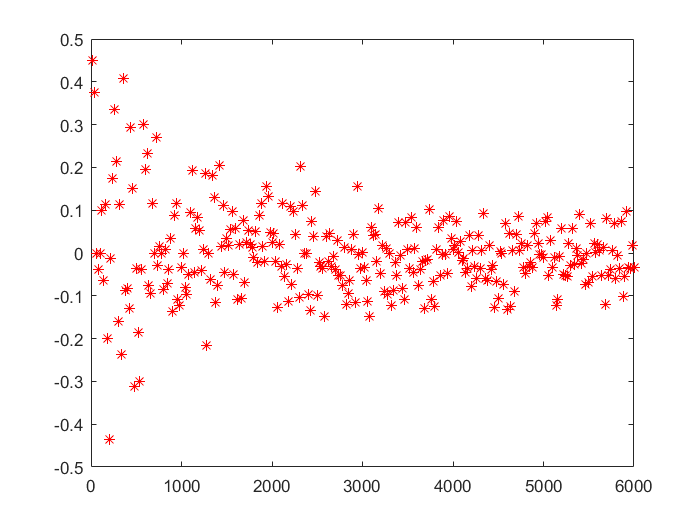
\includegraphics[width=0.6\textwidth, trim = {0 0 0 0},clip]{./ImagenesEjercicio1/media.png}
	\caption{.}
	\label{fig:media}
\end{figure}

\subsection{Conclusiones sobre los resultados}

Podemos concluir que para los valores experimentales, la media en $t_1 = \frac{\pi}{2}$ es cercana a cero y como se puede observar en la figura (\ref{fig:media}) a medida que aumentamos la cantidad de valores muestreados la diferencia entre el valor experimental y el valor teórico es cada vez más pequeña. De igual manera, para la varianza en $t_1 = \frac{\pi}{2}$, no se observan diferencias significativas.
También, la autocorrelación en $t_1 = \frac{\pi}{2}$ y $t_2 = \frac{\pi}{4}$ y la autocorrelación en $t_3 = \pi$ y $t_4 = 2\pi$ denotan el mismo comportamiento hacia el valor teórico. 





\end{document}